\chapter{Related Work}
\label{ch:relatedwork}

Throughout the COVID-19 pandemic, several research studies have explored the application of machine learning and deep learning techniques to deal with the challenge of the infodemic.\\

For instance, Patwa et al.\cite{b4} have focused exclusively on textual English content, disregarding texts in other languages. The datasets were sourced from publicly available fact-checking websites and social media platforms, targeting fake news. In contrast, real news was collected from the Twitter accounts of 14 official and verified government or medical institutions through web crawling. Each article underwent a manual review for accuracy and relevance.
In the preprocessing phase, the collected data was cleaned by removing all links, non-alphanumeric characters, and English stop words. The term frequency-inverse document frequency (TF-IDF) method was employed for feature extraction. Various machine learning algorithms, including Logistic Regression (LR), Support Vector Machine (SVM) with a linear kernel, Decision Tree (DT), and Gradient Boosting Decision Tree (GDBT), were experimented with the TF-IDF feature. These algorithms were implemented using the sklearn package. Among them, the SVM algorithm achieved the highest test F1 score of 93.32\%, closely followed by Logistic Regression with a 91.96\% F1 score.
This approach to data collection, preprocessing, and model experimentation provides a robust foundation for our study, allowing for meaningful comparisons. The approach also demonstrated the ability of machine learning techniques to address misinformation.\\

Similarly, utilizing the same dataset, Das et al.\cite{b5} employed pre-trained language models (PLMs) for preprocessing and training tasks. Their approach combined predictions from multiple models through a soft voting mechanism, showing admirable results, as evidenced by their success in the CONSTRAINT2021 COVID-19 Fake News Detection competition.
In text preprocessing for fake news detection, they have leveraged various Python libraries to filter out colloquial language, usernames, URLs, and emojis. These preprocessing steps ensure the textual data is clean and suitable for model training.
Their study employed a variety of pre-trained language models, including XLNet, RoBERTa, XLM-RoBERTa, DeBERTa, ERNIE 2.0, and ELECTRA. These models utilized pre-trained weights as their initial starting points, which were then fine-tuned on the specific datasets for the classification task. All textual data was tokenized using the tokenizers corresponding to each pre-trained model, ensuring consistency with the model architectures.
Each model was appended with an additional fully connected layer at the bottom to generate prediction probabilities. Moreover, ensemble methods such as soft and hard voting were applied to combine the predictions of the well-performing models. These ensemble techniques aim to ease the limitations of individual models by balancing their strengths and weaknesses, thereby improving overall performance in fake news detection tasks. This study also highlights the effectiveness of advanced pre-trained language models in enhancing the accuracy of fake news detection.\\

Paka et al. \cite {b6} proposed that more than relying on textual features may be required for accurate fake news classification. 
First, they gathered COVID-19-related tweets from Twitter via Twitter API for their dataset. They comprehensively analyzed the dataset, examining the occurrences of major keywords and the distribution of sentiment and likes across the tweets. This analysis provided valuable insights into the characteristics of the tweets related to COVID-19. 
In addition to textual data, Paka et al. incorporated supplementary information such as the number of likes a tweet received, the presence of external links, and the follower count of the users who posted the tweets. These additional features, categorized as tweet features and user features, enriched the textual dataset and contributed to more information for classification.  
They presented an innovative classification approach utilizing a cross-stitch unit in combination with a Long Short-Term Memory (LSTM) architecture (Fig. \ref{fig:Cross-SEAN.}). The cross-stitch unit was employed to handle tweet and user features, while the LSTM was used to process the textual data. These sections were then concatenated via a fully connected layer. This hybrid model architecture demonstrated the potential benefits of integrating diverse features from social media for fake news detection.
The method proposed by Paka et al. achieved an impressive F1-score of 95.3\%, highlighting the effectiveness of incorporating both textual and non-textual features in improving the accuracy of fake news detection.\\

\begin{figure}
    \centering
    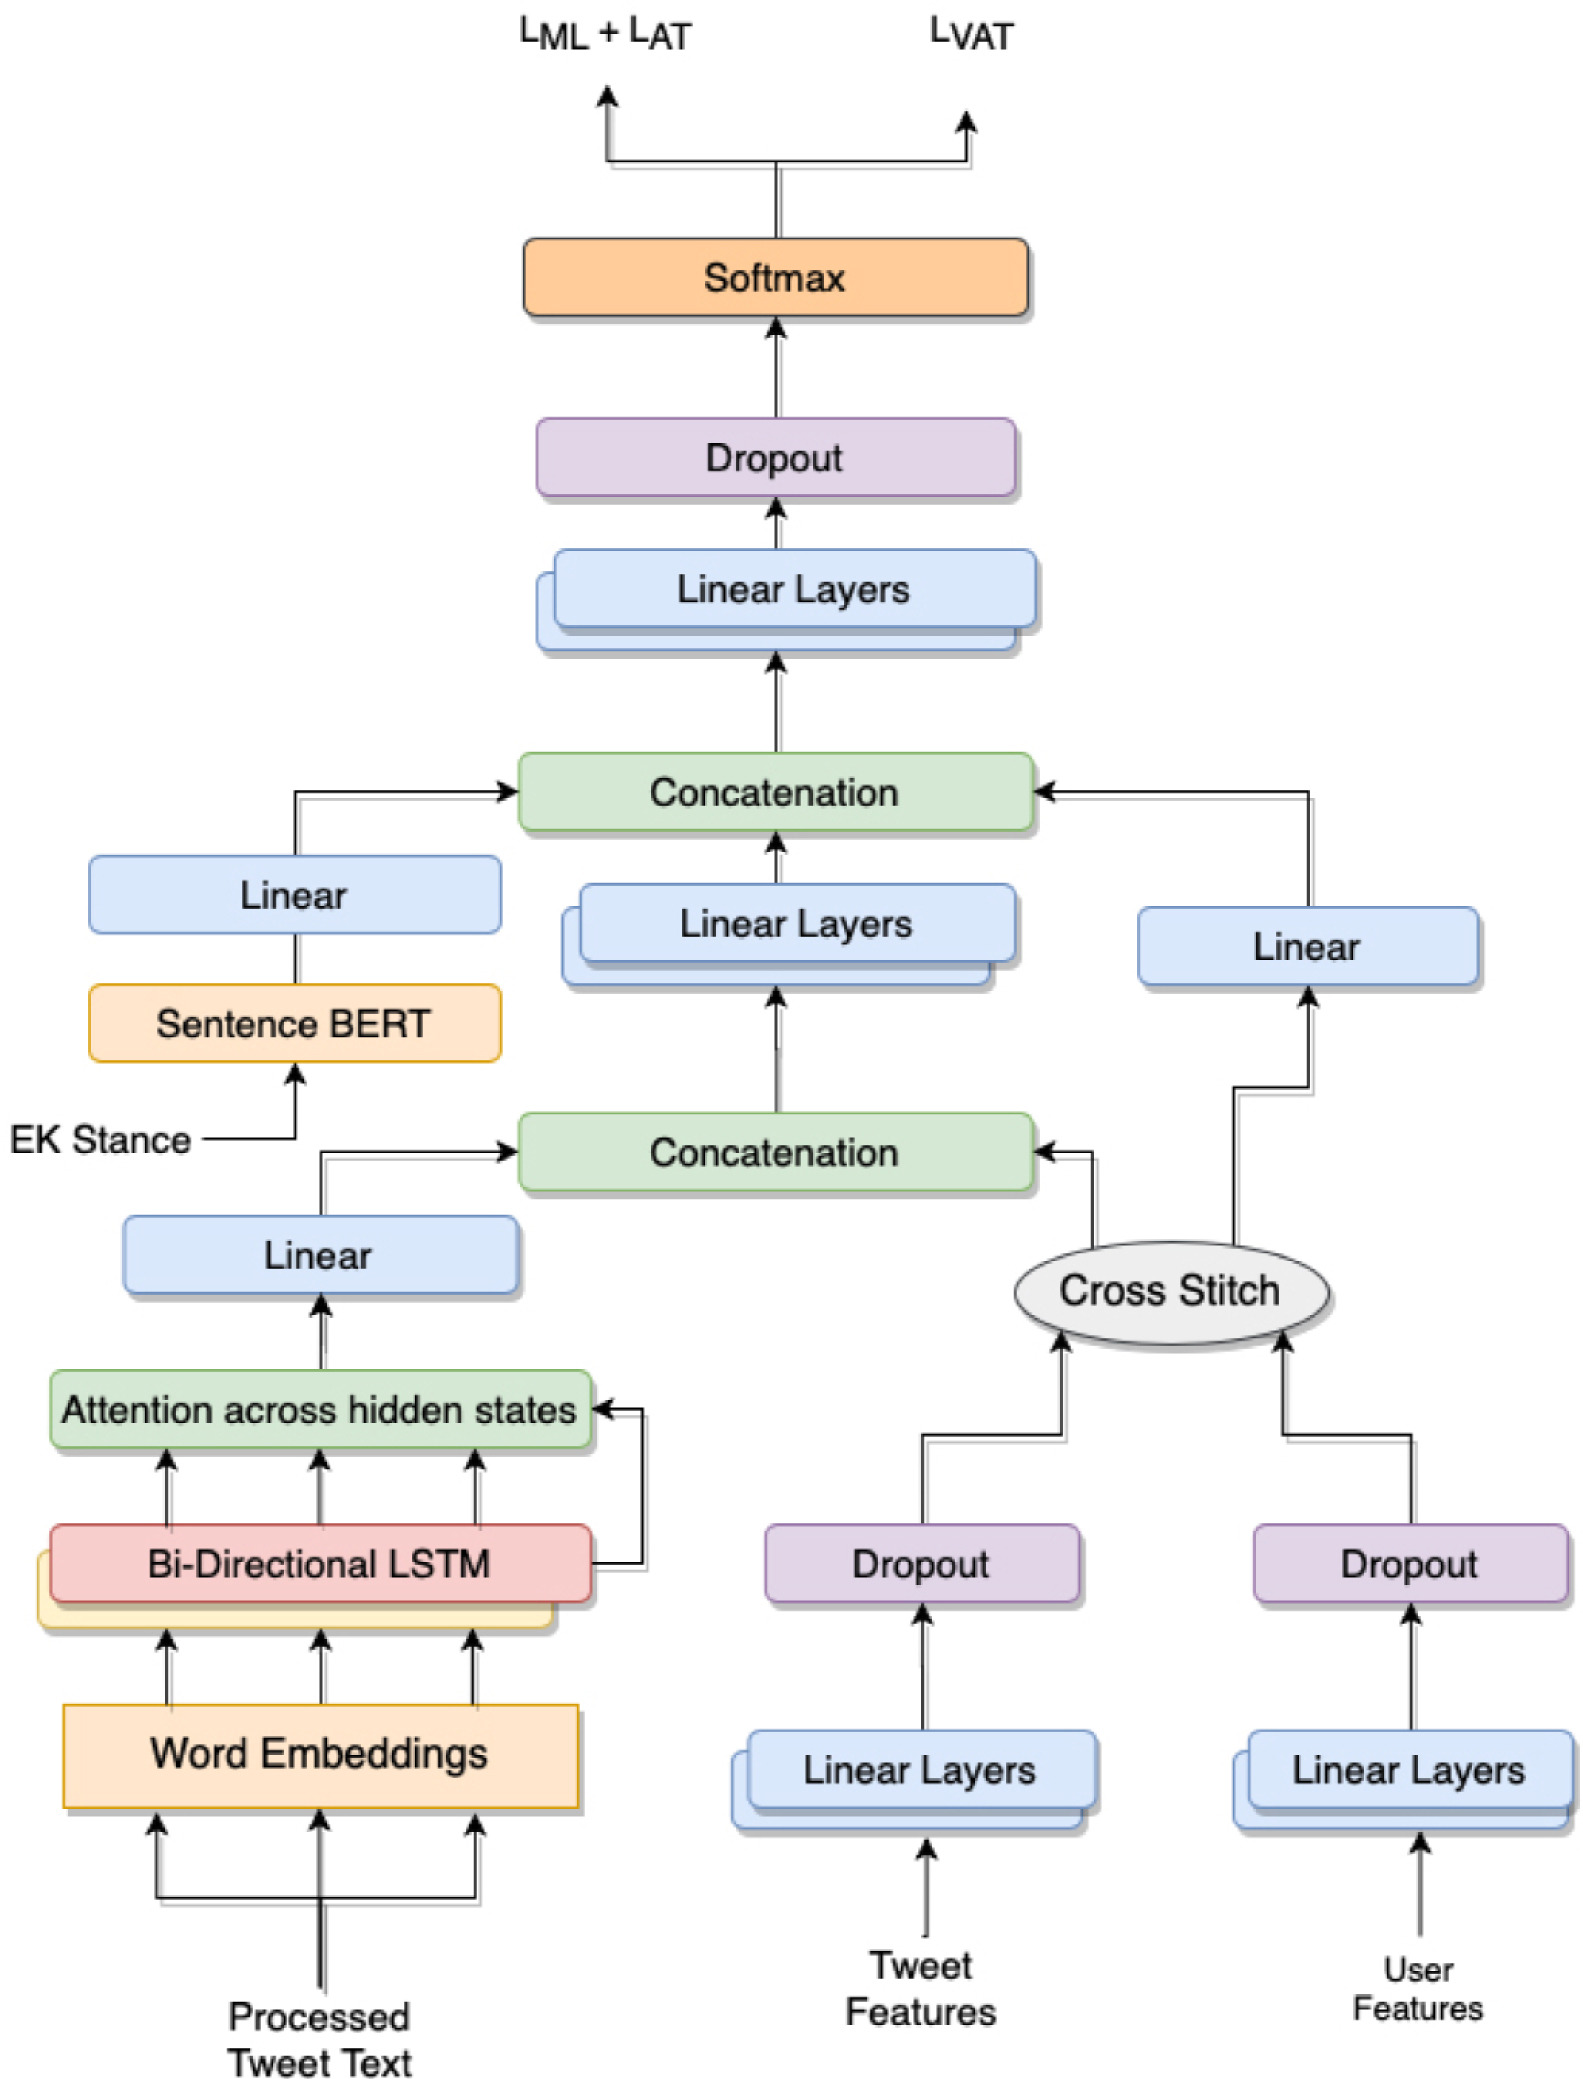
\includegraphics[width=1\linewidth]{img/Cross-SEAN.jpg}
    \caption{The architecture of Cross-SEAN \cite{b6}.}
    \label{fig:Cross-SEAN.}
\end{figure}

Furthermore, research teams focusing on the Chinese language have also made efforts in this domain \cite{b7}. They gathered fact-checked microblogs from Weibo, a popular Chinese social media platform. These microblogs were meticulously labeled and contained various attributes, including blog\_id, date, user\_id, text\_content, number of comments, number of reposts, and number of likes.
Similar to other research, they comprehensively analyzed the collected dataset. The analysis included statistical investigation and the distribution of selected keywords within the dataset (Fig. \ref{fig:CHECKED}). They also presented a visualized word cloud to provide a clearer picture of the prominent terms in the data.
To classify COVID-19 fake news in Chinese text, they utilized advanced deep learning frameworks such as TextCNN and attention-based models like Attention-based TextRNN (Att-TextRNN) and Transformer. These models are well-suited for processing textual data to distinguish between real and fake news.
Their method achieved high performance, with F1-scores reaching 93.8\% with TextCNN and 92.7\% with Transformer. These results underscore the effectiveness of deep learning approaches in handling the intricacies of fake news detection in Chinese text.
These efforts emphasize the global commitment to combating the infodemic.\\
\begin{figure}
    \centering
    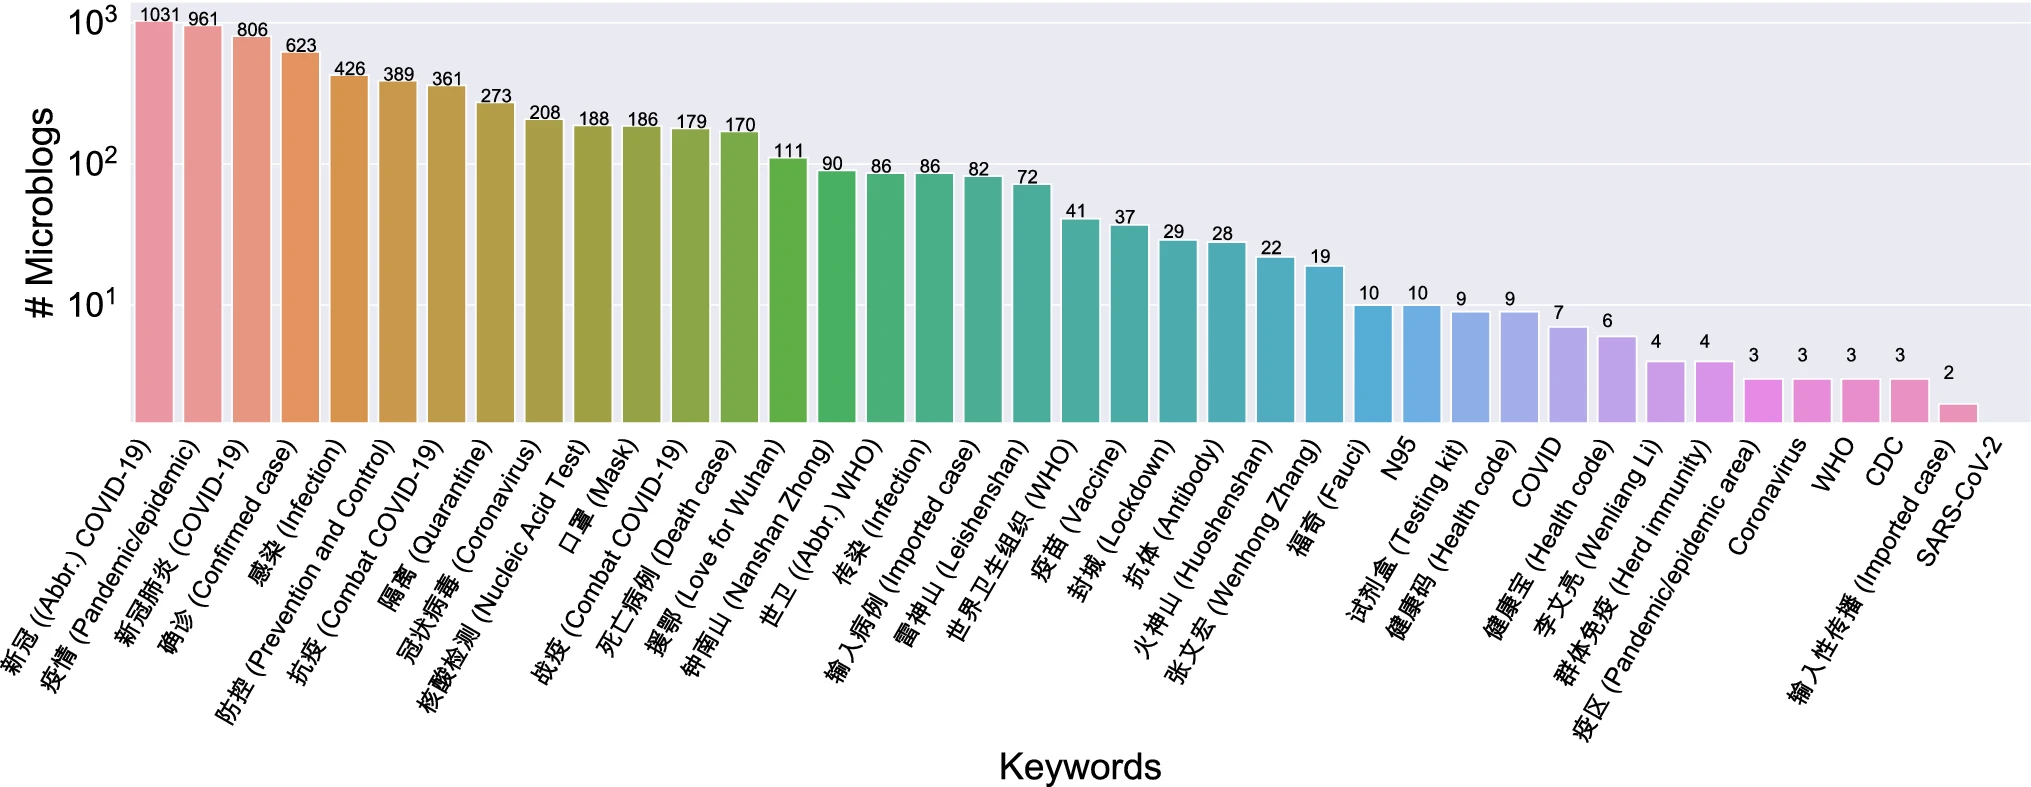
\includegraphics[width=1\linewidth]{img/CHECHED_Keywords.png}
    \caption{Distribution of selected keywords in CHECKED \cite{b7}.}
    \label{fig:CHECKED}
\end{figure}

Additionally, the emergence of large language models (LLMs) based on transformers, such as ChatGPT \cite{b8}, has recently received significant attention. These state-of-the-art models, equipped with advanced natural language understanding capabilities and interactive functionalities, hold enormous potential for developing more powerful tools to combat the spread of misinformation across diverse domains. Their ability to comprehend complex language nuances and engage users in meaningful interactions represents a new stage in advancing fake news detection.
Despite their potential, more studies are needed to explore the capability of LLMs to detect fake news. While LLMs can generate outputs that are coherent and grammatically correct, they may also produce hallucinations (Fig. \ref{fig:Hallucination})—factually incorrect or nonsensical content that appears plausible. This issue raises the importance of evaluating LLMs compared to traditional machine learning algorithms and deep learning models.\\

\begin{figure}
    \centering
    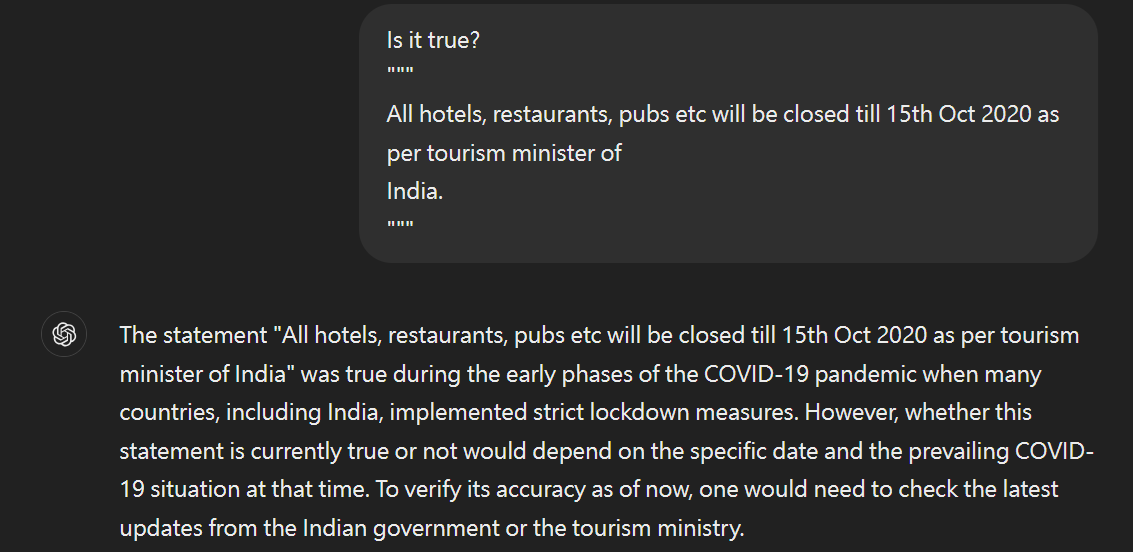
\includegraphics[width=1\linewidth]{img/Hallucination.png}
    \caption{An example of ChatGPT's hallucination, where it incorrectly labels a fake article from a previous study \cite{b4} as true.}
    \label{fig:Hallucination}
\end{figure}
By examining the performance of LLMs against established methods, researchers can better understand the strengths and weaknesses of these models in the context of fake news detection. This comparison is crucial to ensure the reliability and effectiveness of LLMs in real-world applications.